\chapter{Risultati}
In questo capitolo saranno presentati i risultati ottenuti nelle varie
simulazioni. Quando non meglio specificato, i parametri sono stati mantenuti
come indicato nel capitolo relativo alla progettazione.\newline
Visto il nostro assegnamento dei valori di fitness, il punteggio massimo è 100
punti, ottenuto non entrando mai nei muri, non scontrandosi mai con altri robot
e raccogliendo tutte e 10 le lattine. Il punteggio più basso possibile è -5
moltiplicato per il numero di azioni che gli agenti possono compiere,
moltiplicato a sua volta per 2 (per ogni agente sulla mappa).



\section{Vista a Croce Non Collaborativa}
Con la vista a croce non collaborativa i robot non possono vedere il proprio
compagno sulla mappa. Le celle che sono in grado di percepire sono quella a
nord, quella a sinistra, quella nella quale si trovano, quella a destra e quella
a sud.

\subsection{100 Coppie}
La prima simulazione è stata effettuata usando lo schema dell'algoritmo genetico
descritto precedentemente, con un numero di coppie pari a 100, ovvero 200
robot.\newline
In 5000 generazioni il valore di fitness, dopo un primo incremento, si è sempre
mantenuto attorno al valore 0. Questo ci ha fatto supporre che la strategia di
evoluzione da noi adottata dovesse essere modificata. Anziché generare tutti i
nuovi individui mediante l'utilizzo del crossover, abbiamo deciso di copiare
alcuni degli individui vecchi nella nuova generazione, adottando una strategia
élitaria.

\subsection{100 Coppie, da 1 a 5 Vecchie}
\begin{figure}[ht]
	\centering
	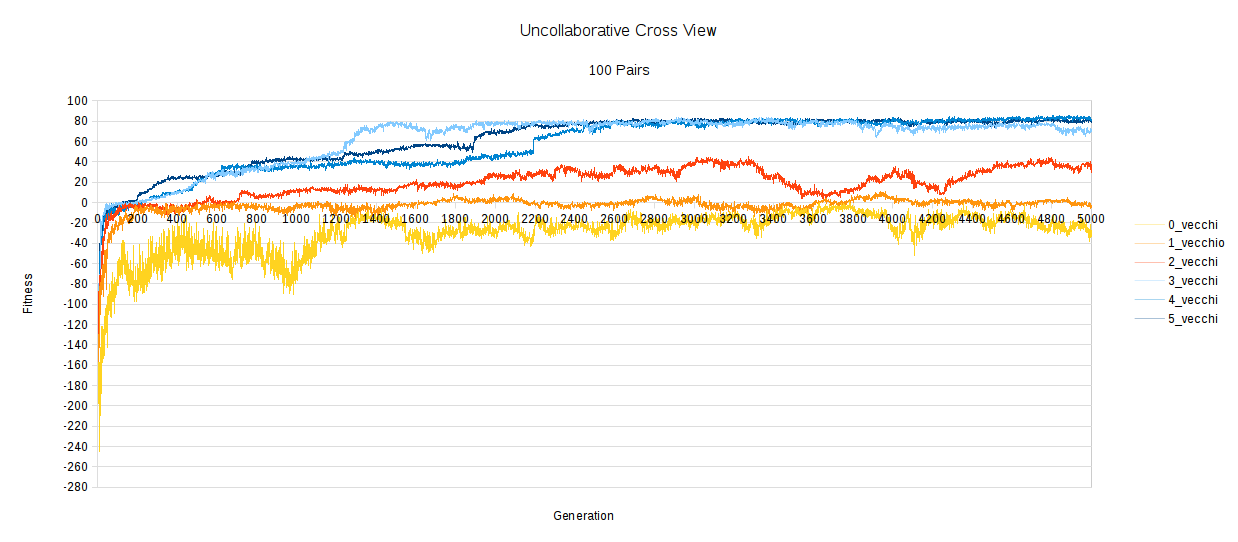
\includegraphics[scale=0.7,angle=90]{imgs/cross_nc_100_pairs_0_5_old.png}
	\caption{Vista a croce non collaborativa, 100 coppie}
	\label{figure:cross_nc_100_0_5}
\end{figure}
La Figura~\ref{figure:cross_nc_100_0_5} mostra i valori di 6 simulazioni nelle
quali abbiamo mantenuto da 0 (tutti gli individui generati tramite l'uso del
crossover) a 5 coppie (le migliori) dalla vecchia alla nuova generazione. Come è
possibile notare, più sono gli individui che vengono mantenuti da una
generazione all'altra, più alto è il valore di fitness raggiunto.

\subsection{100 Coppie, da 10 a 35 Vecchie}
\begin{figure}[ht]
	\centering
	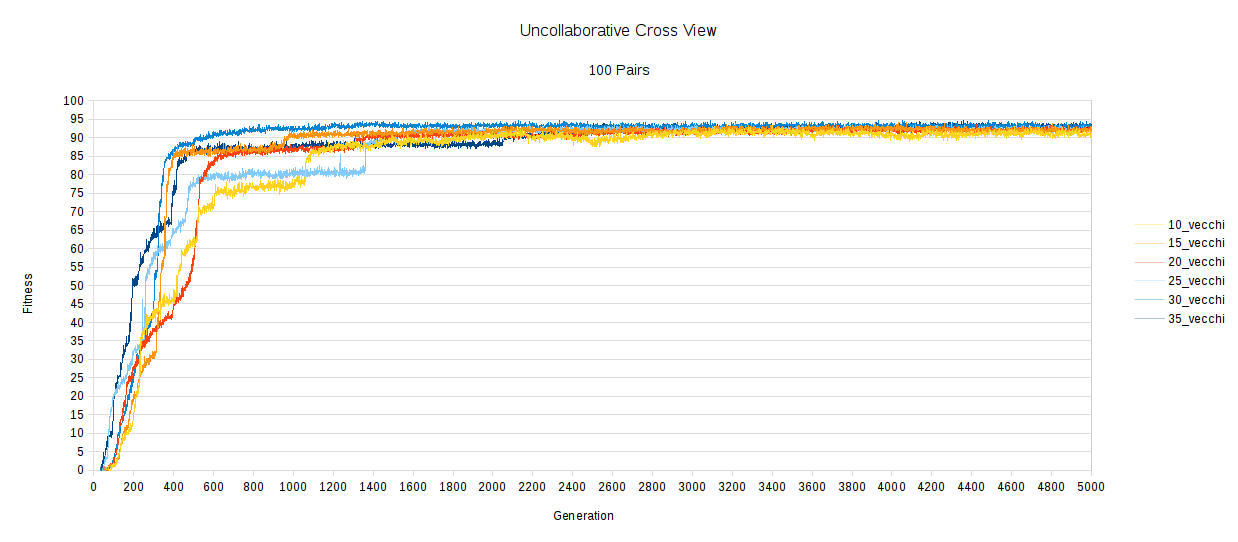
\includegraphics[scale=0.7,angle=90]{imgs/cross_nc_100_pairs_10_35_old.png}
	\caption{Vista a croce non collaborativa, 100 coppie}
	\label{figure:cross_nc_100_10_35}
\end{figure}
In Figura~\ref{figure:cross_nc_100_10_35} abbiamo proseguito con il
ragionamento, copiando nella nuova generazione da 10 a 35 coppie, incrementando
l'intervallo da 1 a 5. I valori di fitness si mantengono tutti fra i 90 ed i 95
punti.

\subsection{100 Coppie, da 40 a 90 Vecchie}
\begin{figure}[ht]
	\centering
	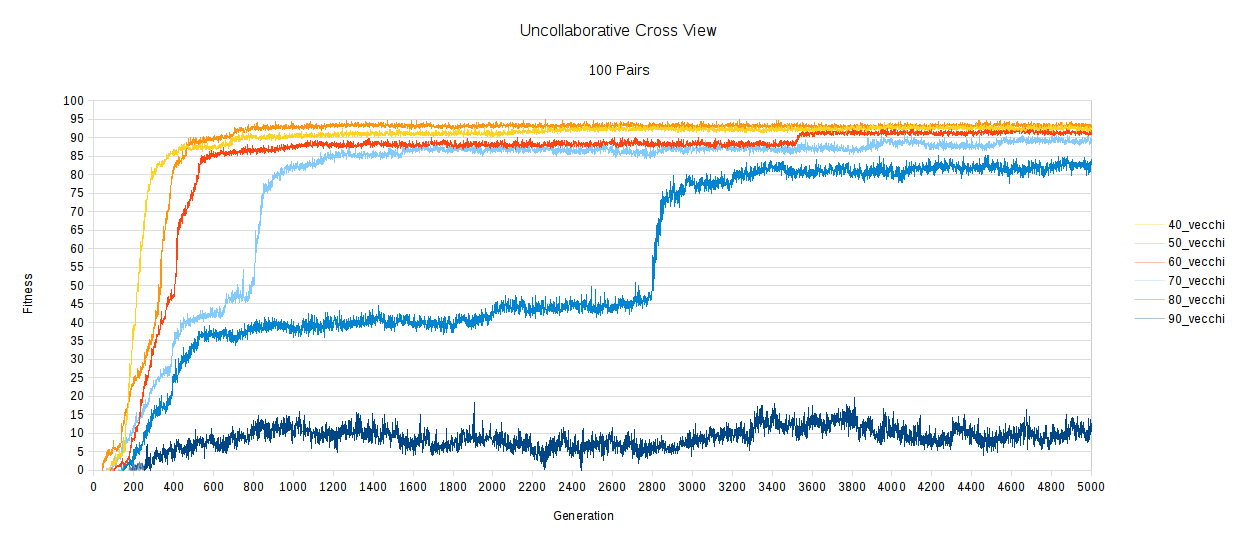
\includegraphics[scale=0.7,angle=90]{imgs/cross_nc_100_pairs_40_90_old.png}
	\caption{Vista a croce non collaborativa, 100 coppie}
	\label{figure:cross_nc_100_40_90}
\end{figure}
A questo punto ci siamo chiesti quando le performance sarebbero crollate ed
abbiamo ulteriormente iterato il procedimento mantenendo da 40 a 90 coppie,
procedendo per intervalli di 10.\newline
Come è mostarto in Figura~\ref{figure:cross_nc_100_40_90}, man mano che il
numero di coppie vecchie passate nella nuova generazione aumenta, il valore di
fitness inizia a scendere, fino a mostrare cali importanti con 80 e 90 coppie.
Mantenendo nella nuova generazione 40, 50 e 60 coppie, comunque i valori di
fitness rimangono fra i 90 ed i 95 punti.

\clearpage

\subsection{200 Coppie, da 10 a 180 Vecchie}
\begin{figure}[ht]
	\centering
	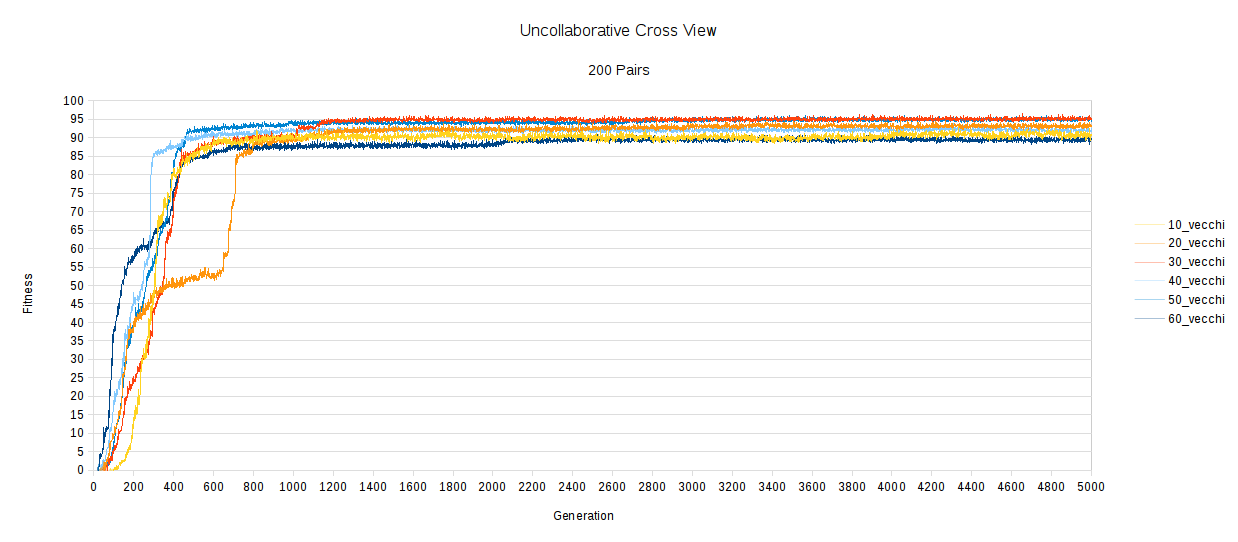
\includegraphics[scale=0.7,angle=90]{imgs/cross_nc_200_pairs_10_60_old.png}
	\caption{Vista a croce non collaborativa, 200 coppie}
	\label{figure:cross_nc_200_10_60}
\end{figure}
\begin{figure}[ht]
	\centering
	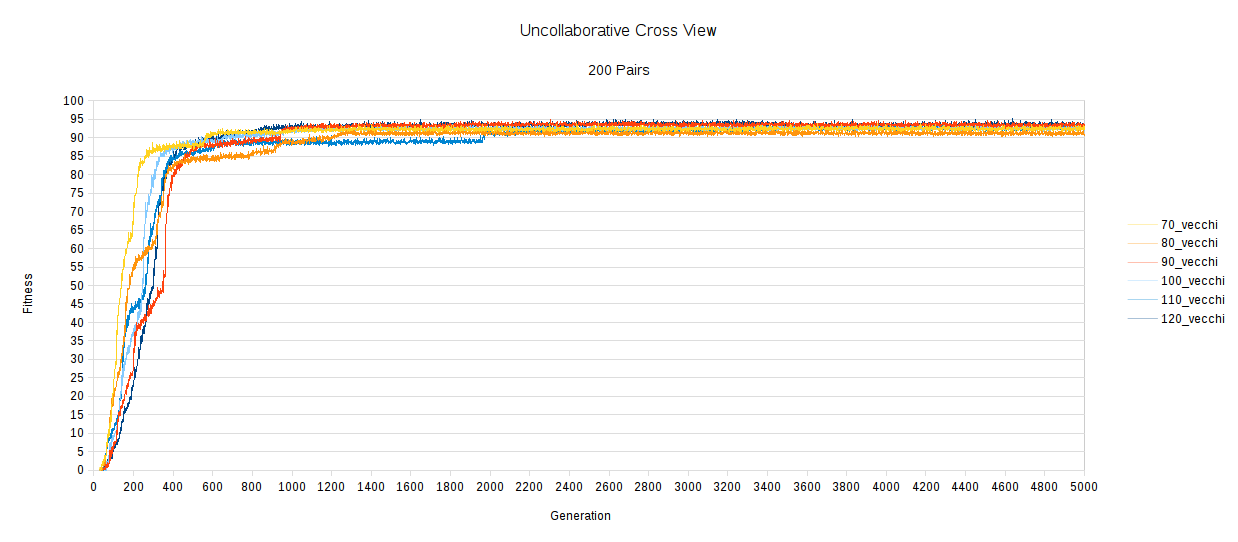
\includegraphics[scale=0.7,angle=90]{imgs/cross_nc_200_pairs_70_120_old.png}
	\caption{Vista a croce non collaborativa, 200 coppie}
	\label{figure:cross_nc_200_70_120}
\end{figure}
\begin{figure}[ht]
	\centering
	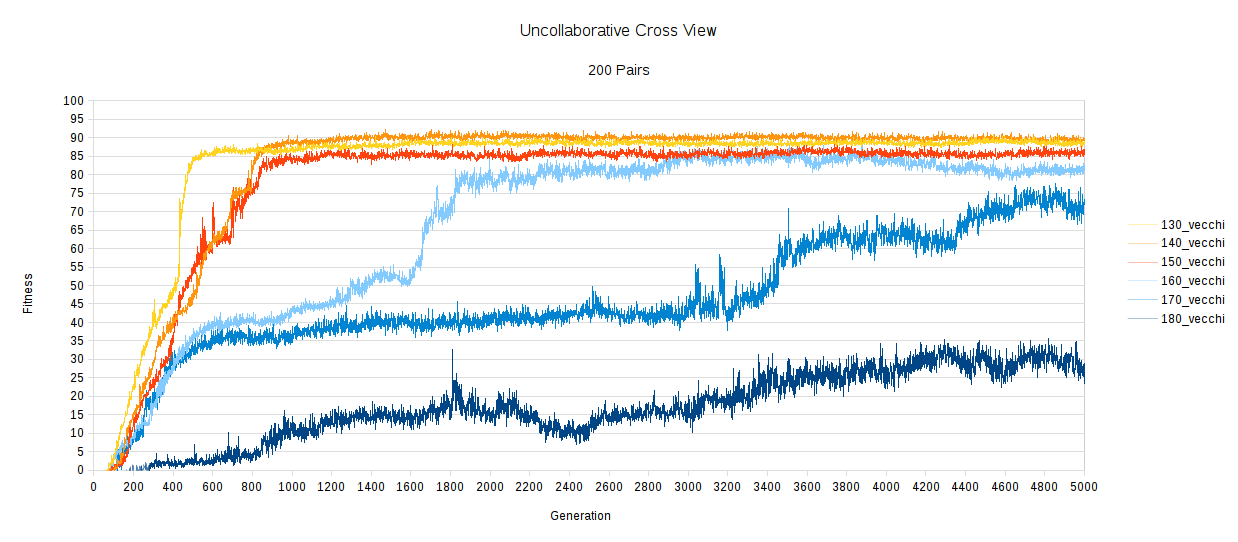
\includegraphics[scale=0.7,angle=90]{imgs/cross_nc_200_pairs_130_180_old.png}
	\caption{Vista a croce non collaborativa, 200 coppie}
	\label{figure:cross_nc_200_130_180}
\end{figure}
Avendo notato come la modifica di un semplice parametro (il numero di coppie
vecchie da mantenere nella nuova popolazione) possa influenzare in maniera
significativa l'evoluzione, abbiamo deciso di ripetere lo stesso procedimento
aumentando il numero di coppie che formano la popolazione da 100 a 200. Così
facendo abbiamo sperato, avendo più varietà genetica all'inizio, di poter
raggiungere valori di fitness più alti.\newline
La Figura~\ref{figure:cross_nc_200_10_60} mostra l'andamento dell'evoluzione
tenendo da 10 a 60 coppie, la Figura~\ref{figure:cross_nc_200_70_120} da 70 a
120 e, infine, la Figura~\ref{figure:cross_nc_200_130_180} grafica l'andamento
dei valori di fitness tenendo da 130 a 180 coppie vecchie nella nuova
generazione.\newline
Per quanto riguarda il raggiungimento di valori di fitness più alti, partire
con una popolazione più grande (di dimensione doppia) non ha dato i risultati
sperati. Se però si notano le velocità con cui le varie curve crescono verso i
valori di fitness più grandi (il numero di generazioni che impiegano a superare,
ad esempio, gli 80/85 punti di fitness), ci si rende conto come avere una
popolazione formata da 200 coppie incrementi di molto le performance.\newline
Questo esperimento ci ha poi permesso di identificare una costante, ovvero, che
i valori di fitness più alti sono raggiunti mantenendo una percentuale
di coppie vecchie da una generazione all'altra che va dal 10\% al 60\%. Con una
popolazione di 100 coppie, infatti, i valori di fitness tra i 90 ed i 95 punti
sono stati raggiunti mantenendo da 10 a 60 vecchie coppie nelle nuove
generazioni, mentre, incrementando il numero di coppie a 200, gli stessi valori
di fitness sono raggiunti mantenendo da 20 a 120 vecchie coppie nelle nuove
generazioni.

\clearpage

\subsection{200 Coppie, da 70 a 120 Vecchie Non Mutate}
\begin{figure}[ht]
	\centering
	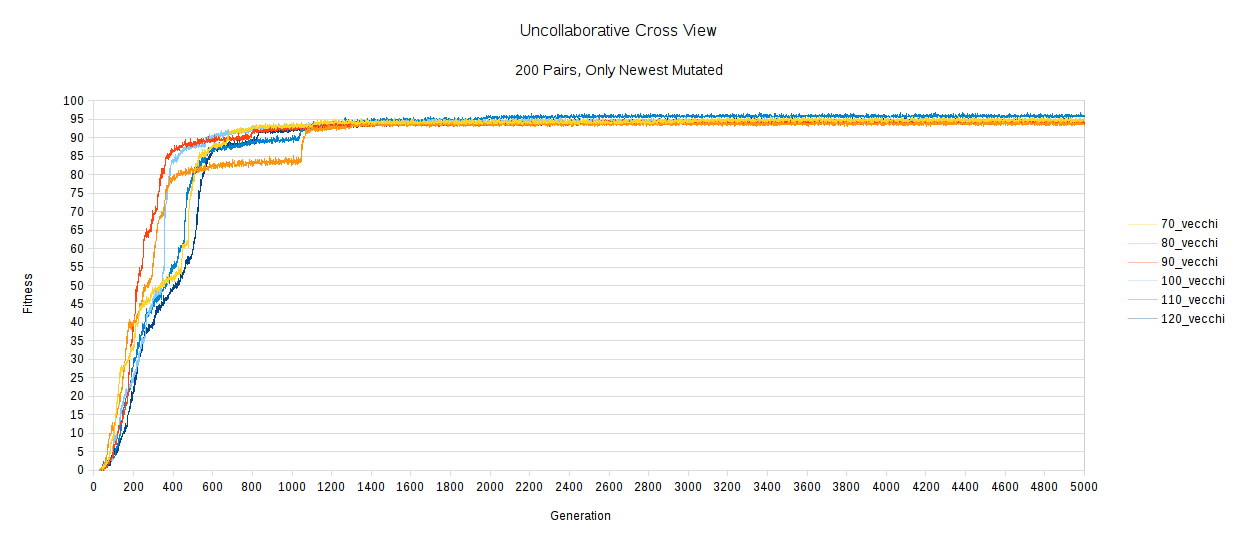
\includegraphics[scale=0.7,angle=90]{imgs/cross_nc_200_pairs_70_120_old_not_mutated.png}
	\caption{Vista a croce non collaborativa, 200 coppie, vecchie non mutate}
	\label{figure:cross_nc_200_70_120_non}
\end{figure}
Abbiamo poi effettuato un'ultima simulazione nella quale abbiamo ripreso il
numero di coppie dalla vecchia alla nuova generazione che meglio si sono
comportate (che hanno raggiunto i valori di fitness più elevati) con popolazione
di dimensione 200 coppie, dove però le mutazioni genetiche sono state applicate
solo ai nuovi individui generati e non più anche ai vecchi.\newline
I risultati sono riportati in Figura
\ref{figure:cross_nc_200_70_120_non}. Confrontando questo grafico con quello di
Figura~\ref{figure:cross_nc_200_70_120}, si nota come la velocità nella crescita
sia paragonabile ma, non mutando le vecchie coppie, i valori di fitness siano
tutti più elevati: questi, infatti, non scendendo mai sotto i 95 punti.



\clearpage



\section{Vista Quadrata Non Collaborativa}
Questo tipo di vista, così come la precedente, non permette ai robot di
percepire la presenza degli altri Robby sulla mappa. A differenza di quella a
croce, però, questa fa sì che i robot possano vedere un numero di celle
maggiore. Sono infatti visibili anche le caselle in alto a sinistra, in alto a
destra, in basso a sinistra ed in basso a destra, trasformando quella che prima
era una croce in un quadrato di 3x3 celle. Come nel caso precedente, il robot
occupa la posizione centrale (seconda riga e seconda colonna).

\subsection{200 Coppie, da 70 a 120 Vecchie Non Mutate}
\begin{figure}[ht]
	\centering
	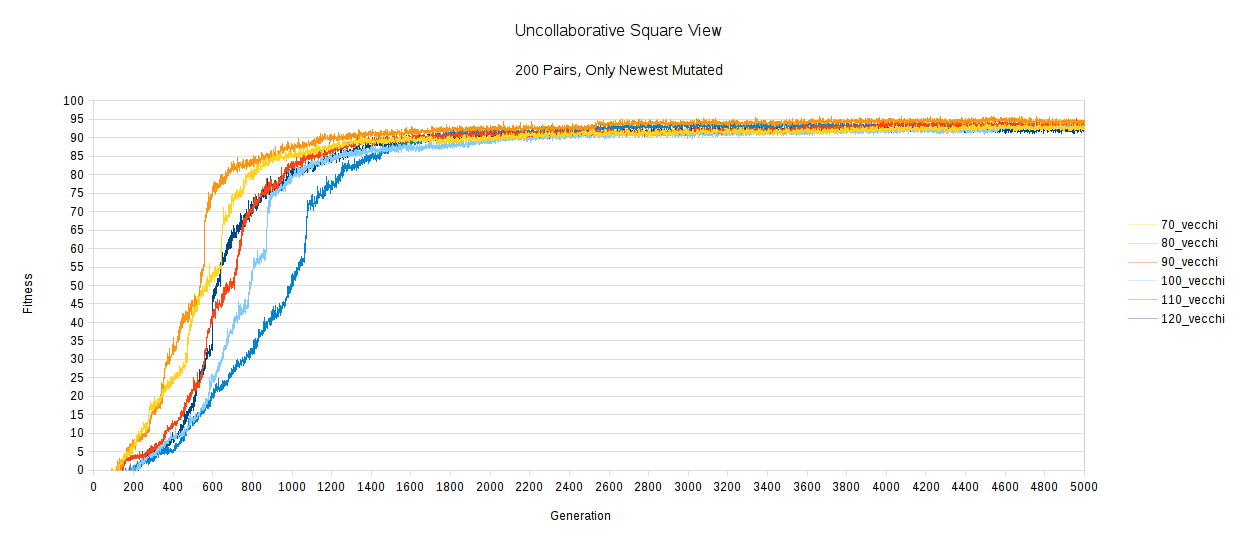
\includegraphics[scale=0.7,angle=90]{imgs/square_nc_200_pairs_70_120_old_not_mutated.png}
	\caption{Vista quadrata non collaborativa, 200 coppie, vecchie non mutate}
	\label{figure:square_nc_200_70_120_non}
\end{figure}
Forti dei risultati ottenuti con le simulazioni precedenti, abbiamo evoluto una
popolazione di 200 coppie tenendo, di volta in volta, da 70 a 120 coppie della
vecchia generazione nella nuova, mutando solamente i nuovi individui generati
con il crossover.\newline
I risultati sono mostrati in Figura
\ref{figure:square_nc_200_70_120_non}. Questo risultato ci ha particolarmente
sorpresi in quanto, a rigor di logica, le entità impegnate nel ripulire la
mappa, potendo vedere di più, avrebbero dovuto migliorare i risultati ottenuti
precedentemente, ma così non è stato. Non ci rimane che concludere che una vista
più grande non permette di migliorare le prestazioni che tengono conto del
numero di lattine raccolte.



\clearpage



\section{Vista a Croce Collaborativa}
Questo tipo di vista è del tutto simile alla croce non collaborativa, con la
differenza, però, che è possibile vedere l'altro robot sulla mappa. Dunque, nel
caso in cui un robot si trovi in una casella facente parte della vista di un
Robby, questo vedrà tale cella come occupata da un robot, sia nel caso in cui
questa sia vuota che nel caso in cui vi sia una lattina. Più semplicemente: la
posizione di un robot in una cella oscura la presenza di un'eventuale lattina ad
un altro robot che osserva tale casella.

\subsection{200 Coppie, da 70 a 120 Vecchie Non Mutate}
\begin{figure}[ht]
	\centering
	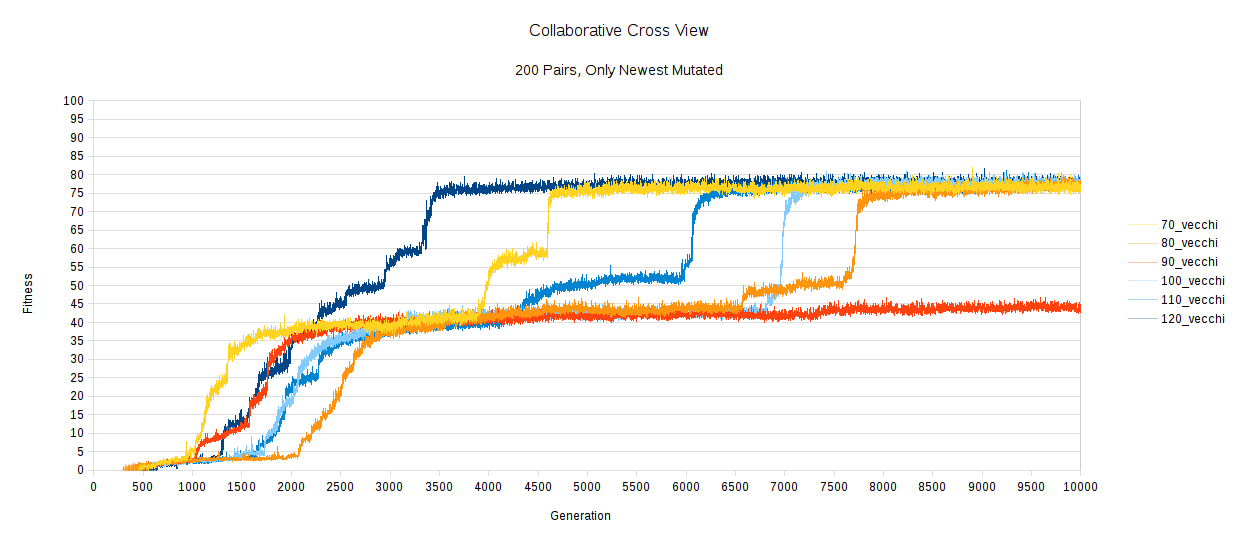
\includegraphics[scale=0.7,angle=90]{imgs/cross_c_200_pairs_70_120_old_not_mutated.png}
	\caption{Vista a croce collaborativa, 200 coppie, vecchie non mutate}
	\label{figure:cross_c_200_70_120_non}
\end{figure}
Dopo aver verificato che il metodo che ha portato i robot con vista non
collaborativa (sia essa a croce o quadrata) ad evolvere nel migliore dei modi 
stato quello che ha adoperato una popolazione formata da 200 coppie mantenendo
dalle vecchie alle nuove generazioni dal 10 al 60\% degli individui, ci siamo
dedicati a riutilizzarlo anche nell'evoluzione dei robot con vista a croce
collaborativa.\newline
Sorprendentemente, però, nonostante sia stato lasciato più tempo ai robot di
evolvere, portando il numero di generazioni da 5000 a 10000, i valori di fitness
si sono mantenuti attorno ad 80. La Figura~\ref{figure:cross_c_200_70_120_non}
riassume i risultati di tali simulazioni.\newline
Oltre a queste simulazioni ne abbiamo fatte di altre, tenendo ad esempio da 10
a 180 coppie vecchie nelle nuove generazioni, sia mutandole che non mutandole e
variando la percentuale di mutazione dallo 0.5\% al 0.1\% (con scatti di 0.1\%),
ma nemmeno modificando questo parametro l'evoluzione è andata meglio.



\clearpage



\section{Viste Non Collaborative a Confronto}
Nelle sezioni precedenti abbiamo visto come evolvendo una popolazione formata da
200 coppie dove ne è mantenuto un certo numero dalla vecchia alla nuova
generazione senza apportarvi modifiche, siano raggiunti in media i 95 punti
fitness. Abbiamo anche visto come dotare i robot di una vista più grande non
permetta loro di ottenere un punteggio maggiore, cioè, raccogliere in media più
lattine.\newline
In questa sezione sono messe a confronto le due viste non collaborative
analizzando se, con un numero di passi minore, quella quadrata 3x3 permetta
almeno di raccogliere lattine più velocemente rispetto a quella a croce. Dunque,
non se sono raccolte più lattine in generale, ma se sono raccolte più
velocemente (con un numero di passi minore).\newline
Per quanto riguarda le strategie evolutive, saranno mantenute quelle che hanno
dato i migliori risultati, ovvero, usando 200 coppie e tenendone invariate dalla
vecchia alla nuova generazione da 70 a 120. Il numero di sessioni usate per
assegnare un valore di fitness medio alla coppia saranno sempre 200, ma verranno
usate solo 30 e 40 azioni (per sessione) anziché 200.

\subsection{40 Azioni}
\begin{figure}[ht]
	\centering
	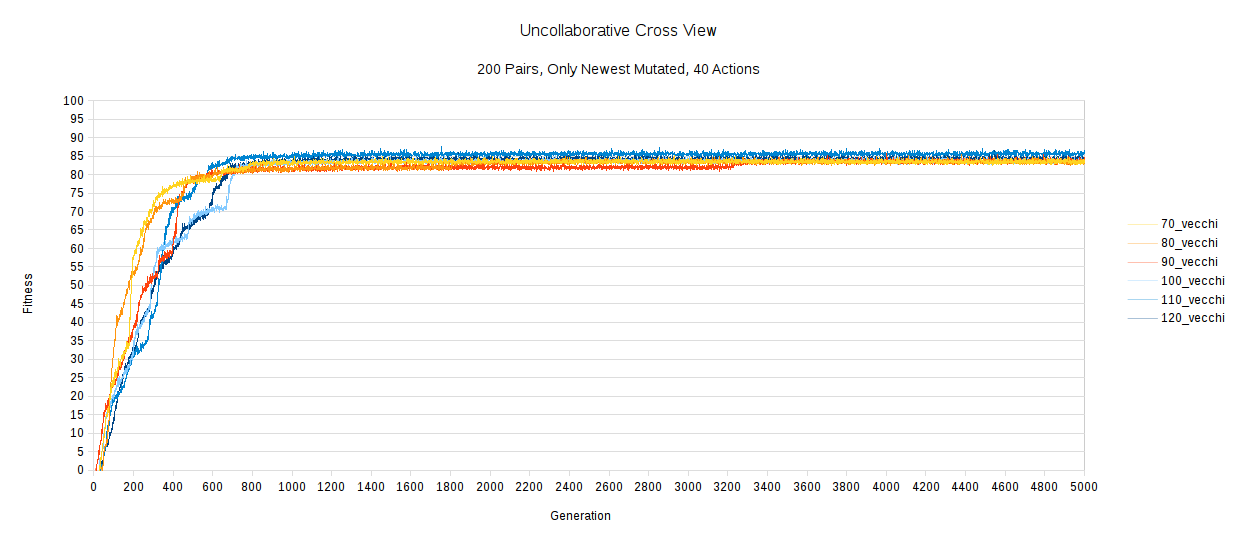
\includegraphics[scale=0.7,angle=90]{imgs/cross_nc_200_pairs_70_120_old_not_mutated_40_actions.png}
	\caption{Vista a croce non collaborativa, 200 coppie, vecchie non mutate, 40 azioni}
	\label{figure:cross_nc_200_70_120_non_40_actions}
\end{figure}
\begin{figure}[ht]
	\centering
	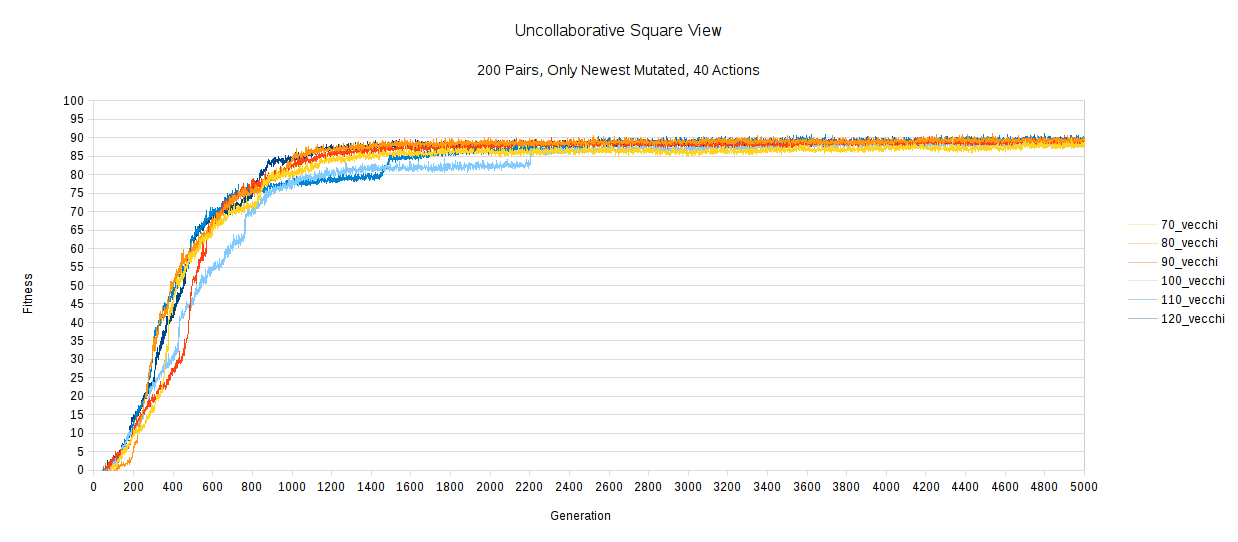
\includegraphics[scale=0.7,angle=90]{imgs/square_nc_200_pairs_70_120_old_not_mutated_40_actions.png}
	\caption{Vista quadrata non collaborativa, 200 coppie, vecchie non mutate, 40 azioni}
	\label{figure:square_nc_200_70_120_non_40_actions}
\end{figure}
Le Figure~\ref{figure:cross_nc_200_70_120_non_40_actions} e
\ref{figure:square_nc_200_70_120_non_40_actions} mostrano gli andamenti delle
evoluzioni usando solamente 40 azioni per sessione. Nel caso in cui sia usata
una vista a croce, i valori di fitness si aggirano attorno ad 85 punti, mentre,
usando una vista quadrata sono toccati i 90 punti.\newline
La vista quadrata sembra iniziare a mostrare la sua superiorità, ma per
confermarlo occorre vedere cosa succede lasciando ai robot ancora meno azioni
per l'apprendimento.

\subsection{30 Azioni}
\begin{figure}[ht]
	\centering
	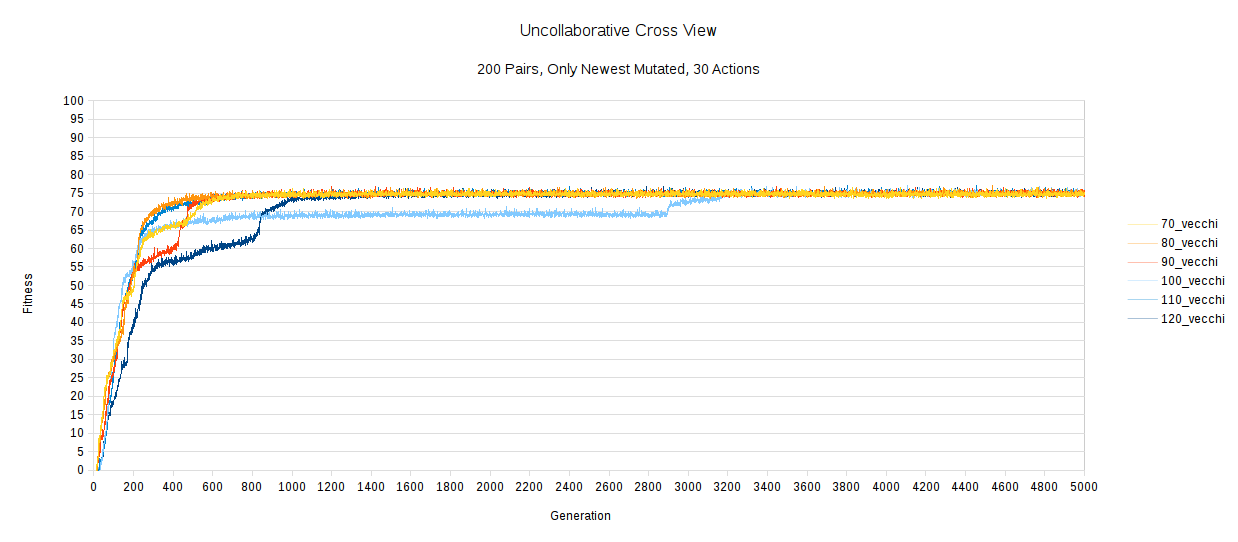
\includegraphics[scale=0.7,angle=90]{imgs/cross_nc_200_pairs_70_120_old_not_mutated_30_actions.png}
	\caption{Vista a croce non collaborativa, 200 coppie, vecchie non mutate, 30 azioni}
	\label{figure:cross_nc_200_70_120_non_30_actions}
\end{figure}
\begin{figure}[ht]
	\centering
	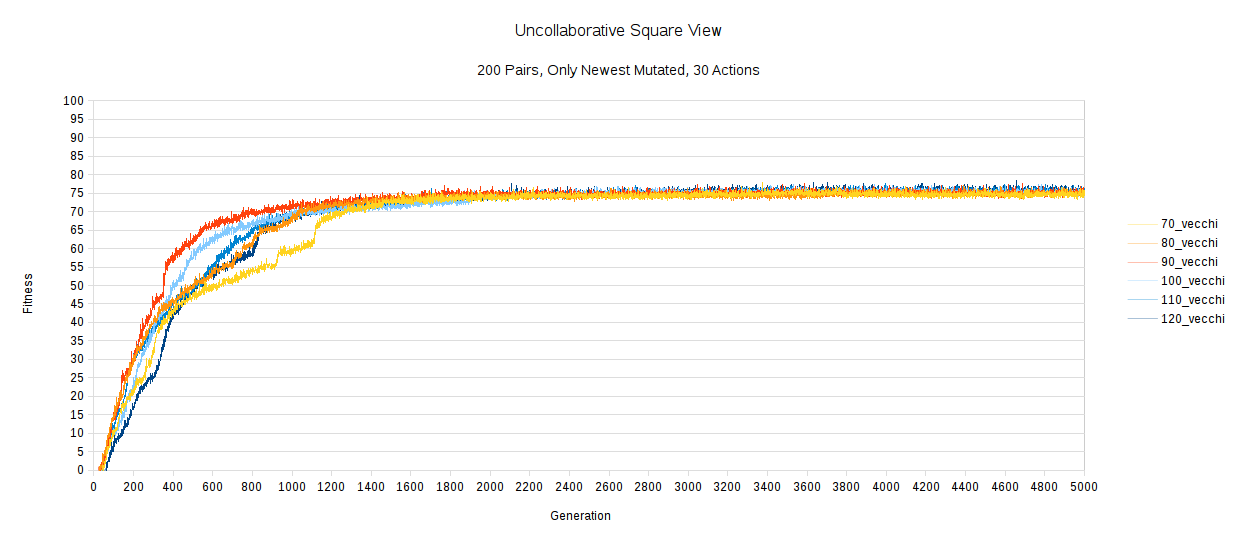
\includegraphics[scale=0.7,angle=90]{imgs/square_nc_200_pairs_70_120_old_not_mutated_30_actions.png}
	\caption{Vista quadrata non collaborativa, 200 coppie, vecchie non mutate, 30 azioni}
	\label{figure:square_nc_200_70_120_non_30_actions}
\end{figure}
Le Figure~\ref{figure:cross_nc_200_70_120_non_30_actions} e
\ref{figure:square_nc_200_70_120_non_30_actions} mostrano come evolve il sistema
impiegando solamente 30 passi. Entrambe le viste si stabilizzano sui 75 punti
fitness.
